% Annoter sur un GPU : extractorAPI

\exapi\footcite{norindrElementExtractionGPU2023} est une \api développée en tant que module de l'application \eida : elle a pour vocation de séparer l'algorithme de détection d'objet du reste de l'application. \exapi est conçue autour d'une unique fonctionnalité : exécuter un algorithme de détection d'objet sur des images reçue de l'application \eida, et retourner les résultats de cette détection.

\subsection{Architecture du système}
    \subsubsection{CPU ou GPU ?}
	L'apprentissage profond et la vision artificielle représentent le plus souvent des tâches qui requièrent une puissance de calcul importante. L'utilisation d'un \gpu plutôt que d'un \cpu est donc de bonne pratique, si ce n'est une nécessité, pour assurer la complétion des tâches en un temps correct, particulièrement lorsqu'il s'agit de tâches qui doivent retourner rapidement un résultat à un utilisateur. Un \gpu est un processeur conçu pour avoir de meilleures performances dans le traitement d'images, et dans l'exécution parallèle de tâches\footcite{sharabokWhyDeepLearning2020}, tandis qu'un \cpu est un processeur conçu pour effectuer des calculs plus basiques, pour répondre aux besoins locaux. Le nombre important de cœurs que contient un \gpu permet une gestion simultanée de nombreuses tâches, et permet donc une plus grande efficacité sur des traitements basés sur le parallélisme, comme le sont les réseaux de neurones, éléments centraux du \dl.
	
	D'un point de vue applicatif, l'utilisation d'un \gpu pour les tâches de vision artificielle permet d'assurer la fluidité du fonctionnement de l'application qui intègre ces algorithmes, et de retourner, comme mentionné précédemment, un résultat rapide à l'utilisateur qui souhaiterait soumettre ses sources à un traitement via l'application. Outre le \ml, un \gpu a les capacités de traiter les images de manière plus performante. Les traitements par des algorithmes de vision artificielle nécessitent en effet un enregistrement des images dans l'application pour que s'effectuent les tâches, ainsi, d'un point de vue matériel, il est essentiel de prévoir, d'une part, la mémoire nécessaire au stockage -- même s'il est temporaire -- des images, ainsi que la puissance de calcul pour leur enregistrement puis leur traitement dans un délai suffisamment court pour retourner une réponse à l'utilisateur en un temps satisfaisant. 
    
    \subsubsection{De l'utilisateur au modèle de détection}
	Les applications \vhs et \eida pour la détection d'objet dans les numérisations reposent sur une même architecture globale, construite pour être adaptable par des projets qui souhaiteraient traiter des sources historiques par la vision artificielle : dans une optique de programmation modulaire, et pour permettre l'utilisation d'un \gpu pour le traitement des images, la solution proposée par ces projets est l'exclusion du modèle de détection de la structure de l'application en elle-même, et le développement d'une \api sur un \gpu pour cette tâche spécifique.
	
	Ainsi, l'application est développée, avec ses dépendances, sur un serveur spécifique, qui accueille le code de l'application et la base de donnée PostgreSQL à laquelle elle est adossée, et stocke les images versées par les utilisateurs qui servent à la génération de manifestes \iiif propres à \eida. Par le biais de l'interface web, l'utilisateur envoie des requêtes à cette application, qui retourne des réponses à l'utilisateur. Le modèle de détection existe sur un serveur indépendant du serveur de l'application, sur un \gpu. Pour connecter le modèle à l'application, une \api est développée : celle-ci reçoit de la part de l'application \eida des requêtes contenant les informations soumises par l'utilisateur, et retourne à l'application une réponse, qui est ensuite retournée à l'utilisateur par son biais. Ainsi, le lien de l'utilisateur au modèle de détection se fait par le biais de l'application, elle-même liée au modèle par une interface qu'est l'\api (fig. \ref{fig:archi_eida}) : l'\api n'a pas d'interface destinée à être vue par l'utilisateur\footnote{Contrairement à l'application, composée d'un \textit{back end} et d'un \textit{front end}, l'\api n'est constituée que d'un \textit{back end}. Il n'existe ainsi pas d'interface accessible à l'utilisateur, seulement le code permettant son fonctionnement.}.
	
	\begin{figure}[h]
		\centering
		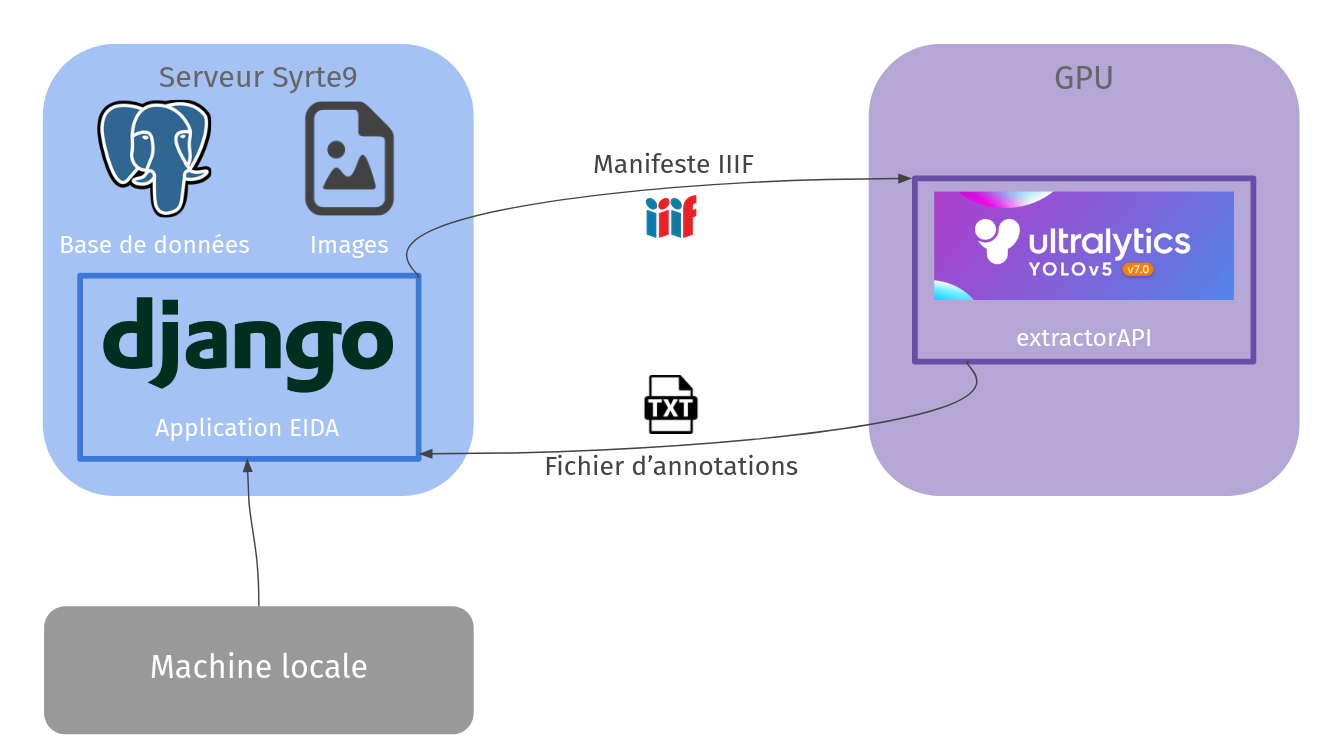
\includegraphics[width=15cm]{images/schema_archi.png}
		\caption{Schéma de l'architecture de l'application \eida et de l'\api \exapi}
		\label{fig:archi_eida}
	\end{figure}

\subsection{Cahier des charges et analyse des besoins}
    \subsubsection{Programmation modulaire et \textit{open source}}
    Avant le développement de l'\api, il est nécessaire d'établir les besoins auxquels cette dernière doit répondre par la rédaction d'un cahier des charges\footnote{Le cahier des charges pour le développement de l'\api a été réalisé lors du premier mois de stage.} (Annexe \ref{exapiCahier}), qui détaille les attentes techniques liées à l'outil créé. La création d'outils \textit{open source} réutilisables par d'autres projets étant un élément central du projet \eida, il est attendu de l'\api qu'elle réponde aux besoins spécifiques du projet tout en présentant la possibilité d'être réemployées dans d'autres contextes. Le lancement d'algorithmes de détection d'objet sur un \gpu est une tâche suffisamment généraliste pour être appliquée par d'autres projets de recherche utilisant la vision par ordinateur pour le traitement des sources historiques ; il est donc souhaitable de créer une \api réemployable pour éviter la multiplication d'outils similaires développés par des projets aux objectifs proches.
    
    Dans cette optique de libre accès, le code de l'\api est mis à disposition sur GitHub, avec la possibilité de le réemployer, en l'adaptant à l'architecture spécifique d'un projet et en modifiant simplement le modèle utilisé pour la détection. La création d'une \api indépendante de l'application \eida renforce la possibilité de remploi des outils développés, puisqu'en tant qu'entité séparée de l'application du projet, l'\api effectue des tâches peu spécifiques, et peut ainsi être intégrée à une application différente sans grandes modifications du code. 
    
    \subsubsection{API REST}
    La communication en \ssh entre le \gpu et l’application \eida n’étant pas satisfaisante du point de vue de la sécurité, le développement d’une \api permet de gérer ces échanges par une voie sécurisée. Il est défini dans le cahier des charges que l'\api communique avec l'application par le biais de requêtes \http qu'elle reçoit et envoie : en tant qu'interface pour la communication de l'application et du modèle de détection, l'\api reçoit des requêtes \http et retourne une ressource spécifique dépendant de l'\URL à laquelle la requête est envoyée.
    
    Par définition, l'\api développée est donc une \api \rest. \rest définit un ensemble de contraintes architecturales pour le développement de services web, qui permettent la communication et l'échange de données sur Internet. Les \api \rest sont basées sur des ressources localisées par des \URL\footcite{APIRESTEst} : lorsqu'un client demande une ressource, il envoie une requête \http\footnote{Les actions à effectuer sur la ressource sont définies par la requête \http : dans ce mémoire, nous mentionnons spécifiquement les requêtes GET, qui permettent au client de récupérer des données, et les requêtes POST, qui permettent d'envoyer des données avec la requête.} à un \textit{endpoint}\footnote{Un \textit{endpoint}, ou point de terminaison, est un emplacement numérique, correspondant à une ressource ou à un service, qui reçoit et envoie des requêtes.} de l'\api, qui retourne en réponse à cette requête une ressource dans un format standard\footnote{Le format \json, par exemple, est un format lisible et interprétable par les machines comme par les humains : il est le plus communément utilisé. \cite{APIRESTEst}}. Dans une \api \rest, les communications entre client et serveur sont \textit{stateless}, signifiant que les informations du client ne sont pas stockées entre les requêtes, et que les requêtes sont traitées indépendamment\footcite{APIRESTEst}. Les \api \rest reposent également sur une interface uniforme pour les interactions avec le client, et un système de couches qui assurent la flexibilité de l'\api et la sécurité des serveurs.
    
    Ainsi, une \api \rest permet la création de services web interopérables : elle facilite la communication entre différents systèmes informatiques en utilisant des requêtes \http pour accéder et manipuler des ressources. Ce mode d'échange des données étant standardisé, il est envisageable pour des projets futurs d'intégrer l'\api à leurs développements, à la seule condition que soit développée une application envoyant des requêtes en accord avec le protocole \http, apte à recevoir des requêtes de la part de l'\api. L'architecture \rest étant pensée pour l'uniformisation et l'intéropérabilité, un grand nombre d'applications sont construites autour de ces principes, et de nombreux \textit{frameworks} les prennent en compte dans les outils qu'ils proposent.
        
    \subsubsection{Sécurité et robustesse}
    Le cahier des charges rédigé en amont du développement de l'\api définit les contraintes du point de vue de la sécurité, des fonctionnalités souhaitées et des échanges de données. \exapi répond ainsi aux besoins spécifiques du projet et de l'application \eida, tout en en faisant le choix d'outils libres, standardisés, qui lui assurent d'être réutilisable dans des contextes et architectures variés.
    
    L'\api, déployée sur un \gpu mis à disposition de l'Observatoire de Paris, se doit d'être sécurisée, pour interdire les requêtes provenant de sources non-identifiées, et éviter ainsi un risque de surcharge de l'\api par des requêtes externes. Une authentification avec un token basée sur les principes \rest\footcite{grinbergRESTfulAuthenticationFlask} a été envisagée, ainsi qu'une restriction des hôtes autorisés à envoyer des requêtes aux \textit{endpoints} de l'\api.
    
    La question de la robustesse est également soulevée parmi les besoins fondamentaux en amont du développement : l'\api est une interface pour des algorithmes appliquant des traitements à des fichiers volumineux -- des images -- en grand nombre, et doit donc avoir la robustesse nécessaire pour accomplir ces tâches. En effet, l'\api reçoit des numérisations d'ouvrages sous la forme de manifestes \iiif, qui représentent ainsi plusieurs centaines d'images à enregistrer avant d'en extraire les objets. Les tâches de lecture du manifeste, d'extraction et d'enregistrement des images sont particulièrement chronophages, tout comme la détection d'objet, il est donc nécessaire de prévoir un gestionnaire de tâches, qui crée une file d'attente des requêtes reçues, afin que ces requêtes successives se lancent dans leur ordre de réception par l'\api, et que le traitement d'une nouvelle source ne se lance qu'après complétion du traitement de la source précédente. Le gestionnaire des tâches permet ainsi d'éviter la surcharge de l'\api en cas de requêtes simultanées, et assure son bon fonctionnement, un temps de traitement correct et une gestion cohérente des requêtes.
    
    Le mode de communication, la sécurité et la robustesse sont trois points fondamentaux du développement applicatif, qui représentent les attentes principales détaillées dans le cahier des charges pour le développement de l'\api. L'objectif d'\exapi est de proposer une structure flexible et légère pour l'inférence d'un modèle de vision artificielle sur un \gpu, afin d'extraire la détection d'objet de l'application du projet, pour en faire un module externe aisément modifiable, réutilisable, et adaptable à des modèles de détection, architectures et besoins variés.
	
\subsection{Développement de l'API}
	\subsubsection{Choix du \textit{framework} : Flask, Django ou FastAPI ?}
	Il existe divers \textit{frameworks}\footnote{Un \textit{framework}, littéralement \og cadre de travail \fg est une bibliothèque de composants logiciels ayant pour vocation à servir de base, ou de squelette, pour le développement d'une application dans un langage donné. Les \textit{frameworks} ont pour vocation de simplifier le travail des développeurs, tout en uniformisant les applications produites.} Python permettant le développement d'une \api. Ces \textit{frameworks} présentant tous des fonctionnalités spécifiques, la première étape du travail de développement d'\exapi est la sélection du \textit{framework} qui servira de squelette à l'application. Trois options ont été envisagées : Django\footcite{Django}, Flask\footcite{FlaskDocumentation} et FastAPI\footcite{FastAPI}.
	
	Django est un \textit{framework} développé en 2003 dédié au développement applicatif en Python, gratuit et en libre accès. L'application \eida, avec laquelle communique \exapi, est basée sur ce \textit{framework}, qui constitue ainsi une option logique dans la continuité du développement de l'application du projet. Les ressources en ligne pour l'intégration de PyTorch, module de \ml, à une application Django sont nombreuses\footcite{arslanCreateMachineLearning2021}, et il existe un \textit{framework} \rest\footcite{DjangoRESTFramework} qui simplifie le développement d'une \api à partir de Django. Apprécié pour sa robustesse, Django est cependant un \textit{framework} assez lourd, constitué de nombreux modules intégrés qui tendent à le ralentir\footcite{sandyChoosingDjangoFlask}. Django permet la création d'\api puissantes, avec des modules nombreux ; cependant, pour le développement d'une \api dont la priorité est la rapidité et la flexibilité, il existe des \textit{frameworks} plus légers, tels que Flask.
	
	Flask est un \textit{framework}, basé sur Django, pour le développement web en Python, basé sur un noyau simple dont les fonctionnalités peuvent être étendues. Minimaliste dans ses modules de base, les principes fondateurs de Flask sont la légèreté et la flexibilité, qui en font un \textit{framework} aisément adaptable à de nombreux projets, simple à prendre en main, et aux possibilités variées. \exapi ayant pour vocation d'être un module léger complémentaire à l'application \eida, il a été choisi d'utiliser Flask pour son développement, afin de produire une \api simple et flexible, qu'il serait aisé d'adapter à d'autres projets, ou aux étapes futures d'\eida, qui impliquent des modèles de vision artificielle aux objectifs différents des modèles de détection utilisés à ce stade.
	
	Le \textit{framework} FastAPI a également été envisagé pour le développement d'\exapi. Ce dernier ayant été publié en 2018, il intègre des fonctionnalités facilitant la rédaction de documentation\footcite{FastAPIFrameworkPython2023} pour l'\api développée, et est réputé pour sa rapidité\footcite{sandyChoosingDjangoFlask}. Sa flexibilité rendait ce \textit{framework} adapté au projet \eida et aux attentes entourant \exapi. Cependant, s'agissant d'un outil récent, la documentation comme la communauté ne sont pas aussi riches que pour les \textit{frameworks} précédemment mentionnés, il a donc été décidé de favoriser Flask pour ce projet, pour permettre un développement fluide et une mise à disposition rapide de l'\api.
	
	\subsubsection{Intégration du modèle de détection}
	L'application \eida et \exapi ayant, en premier lieu, pour vocation d'être des outils à la constitution de jeux de données d'entraînement et de vérité de terrain, il n'existe pas à ce jour de modèle de détection d'objet définitif à intégrer à l'\api. Dans son développement, il est donc nécessaire de prévoir la possibilité de choisir le modèle de détection utilisé, afin de substituer les modèles temporaires utilisés actuellement\footnote{Les modèles utilisés actuellement ne sont pas entraînés sur les données du projet, mais permettent de fournir aux chercheurs qui créent les données d'entraînement une première annotation imparfaite, qu'ils corrigent depuis l'interface d'annotation de l'application, accélérant le travail de création de cette vérité de terrain.} par un modèle entraîné lorsque l'étape d'entraînement sera complétée.
	
	Le script d’inférence utilisé est celui de \yolov\footnote{Il s'agit du script \texttt{detect.py} disponible en accès libre dans le dépôt GitHub du projet. \url{https://github.com/ultralytics/yolov5/blob/master/detect.py}}, reproduit et importé comme un module dans le code de l'\api, et appelé par une fonction lorsque le client envoie une requête à l'\textit{endpoint} servant à la détection d'objet. Le code de \yolov étant en accès libre, le script pour le lancement de la détection est réutilisé avec de légères modifications (Annexe \ref{yoloScript}), et comporte donc les options liées aux fichiers vidéo que \yolo propose initialement : la restriction des formats envoyés est gérée par l'application, qui ne supporte que les manifestes \iiif, les fichiers PDF et les fichiers image, qui sont transmis à l'\api sous forme de manifestes \iiif au format \json. Par défaut, le script fait appel à un modèle de détection \yolov générique, défini par le paramètre \texttt{weights} de la fonction \texttt{run\_vhs} : l'appel à un modèle personnalisé est défini dans les routes de \api\footnote{Les routes sont définies dans le fichier \texttt{app.py} : l'\api ne contenant que deux routes, une architecture simple a été choisie, et les routes ne sont donc pas dissociées du corps du code. \url{https://github.com/jnorindr/extractorAPI/blob/main/app.py}}.
	
	La route correspondant à l'\textit{endpoint} \texttt{/run\_detect} (fig. \ref{fig:run_detect_exapi}) est utilisée pour soumettre une numérisation à traiter par le modèle : recevant de la part de l'application des requêtes \http POST contenant des données, celle-ci prévoit la réception de l'\URL d'un manifeste \iiif contenant les images à annoter, ainsi que le nom du fichier contenant le modèle à utiliser pour la détection. Elle permet ainsi, lors du paramétrage des échanges entre l'application et l'\api, de déterminer le modèle utilisé pour la détection d'objet.
	
	\begin{figure}[h]
		\begin{lstlisting}[language=Python]
		@app.route("/run_detect", methods=['POST'])
		def run_detect():
		# Get manifest URL from the request form
		manifest_url = request.form['manifest_url']
		model = request.form.get('model')
		
		# function.delay() is used to trigger function as celery task
		detect.delay(manifest_url, model)
		return f"Run detect task triggered with Celery! Check terminal to see the logs..."\end{lstlisting}
		\caption{Fonction de la route recevant des requêtes POST contenant une numérisation sur laquelle performer la détection d'objet}
		\label{fig:run_detect_exapi}
	\end{figure}

	La fonction \texttt{run\_detect()} fait appel à une fonction \texttt{detect()} de préparation au lancement de la détection, lancée en tâche de fond, dans laquelle la ligne de code suivante permet d'établir l'utilisation d'un modèle par défaut si aucun modèle spécifique n'est défini dans le formulaire envoyé à l'\textit{endpoint} par l'application (fig\ref{fig:model_exapi}).
	
	\begin{figure}[h]
		\begin{lstlisting}[language=Python]
		model = DEFAULT_MODEL if model is None else model\end{lstlisting}
		\caption{Fragment de code de la fonction \texttt{detect()}}
		\label{fig:model_exapi}
	\end{figure}

	Le modèle par défaut est défini dans le module d'utilitaires de l'\api\footnote{Parmi les utilitaires, le fichier \texttt{path.py} permet de définir les chemins dans l'application, et de les appeler en minimisant le risque d'erreurs. \url{https://github.com/jnorindr/extractorAPI/blob/main/utils/paths.py}}, et permet d'éviter une erreur si le modèle de détection n'est pas défini dans la requête envoyée par le client. La fonction \texttt{detect} fait ensuite appel à la fonction \texttt{run\_vhs}\footnote{Cette fonction correspond au script d'inférence de \yolov.} (fig. \ref{fig:run_vhs_exapi}), avec pour paramètres les informations envoyées dans le formulaire de la requête POST à l'\textit{endpoint} de détection, ainsi que les chemins des images sur enregistrées sur lesquelles performer la détection d'objet, et le chemin du fichier dans lequel doivent être écrites les annotations.
	
	\begin{figure}[h]
		\begin{lstlisting}[language=Python]
			run_vhs(
				weights=f"{MODEL_PATH}/{model}",
				source=wit_path / img,
				anno_file=anno_file,
				img_nb=i
			)\end{lstlisting}
		\caption{Fragment de code de la fonction \texttt{detect()} appelant la fonction \texttt{run\_vhs()} lançant la détection par le modèle}
		\label{fig:run_vhs_exapi}
	\end{figure}

	Ainsi, plusieurs modèles de vision artificielle peuvent être importés sur le \gpu, dans le dossier de l'\api, au format \texttt{.pt}\footnote{Le format \texttt{.pt} est un format standard pour les modèles de \ml créés avec PyTorch. \cite{dowlingGuideFileFormats2019}}. Ces modèles peuvent ensuite être appelés par le script dédié au lancement de l'inférence, avec des paramètres établis dans la requête envoyée par l'application \eida à l'\textit{endpoint} d'\exapi qui reçoit des numérisations pour leur traitement par l'algorithme de détection.

	\subsubsection{Formats des fichiers et échanges de données avec l'application}
	\exapi échange des données avec \eida dans des formats spécifiques, définis dès le cahier des charges, pour correspondre notamment aux exigences de formats pour l'entraînement d'un modèle. 
	
	L'\api reçoit de la part de l'application une requête POST contenant un manifeste \iiif, au format \json, qui permet d'échanger rapidement et de manière efficace des numérisations comportant un grand nombre d'images. Bien que les images de ces numérisations soient enregistrées dans l'application \eida après leur soumission par l'utilisateur, il n'est en effet pas envisageable d'envoyer par requête \http à l'\api un tel volume de fichiers image qui, en plus de représenter plus d'une centaine de fichiers par numérisation, sont des fichiers lourds. L'envoi de manifestes \iiif implique, après réception de la requête par l'\api, l'enregistrement des images sur le \gpu, qui constitue un traitement chronophage mais nécessaire pour la détection d'objet qui ne peut s'effectuer que sur des fichiers image enregistrés\footnote{Il est peu satisfaisant, en termes de performances et de gestion de la mémoire, d'enregistrer les images une première fois sur le serveur de l'application \eida, puis de les enregistrer une seconde fois sur le \gpu. Cependant, à ce jour, aucune chaîne de traitement ne nécessitant qu'un seul enregistrement des images ne s'est avérée satisfaisante -- des réflexions sont actuellement en cours pour modifier cette manière de procéder pour la rendre plus efficace.}. Pour plus d'efficacité, les images ne sont pas supprimées après l'étape de détection d'objet : celles-ci sont conservées pour permettre le lancement rapide de la détection en cas de nouvelle requête envoyée par le client pour une même numérisation. Cependant, le corpus traité par un projet tel qu'\eida représentant des plusieurs centaines -- ou plusieurs milliers -- de numérisations, il est nécessaire de prendre en compte la question de l'espace de stockage sur le \gpu utilisé pour la détection ; ainsi, une fonction avec une tâche périodique, planifiée avec \texttt{crontab}\footnote{\texttt{cron} est un programme permettant d'exécuter des tâches à une heure spécifique, selon un cycle spécifié à l'avance. \cite{Cron2023}}, supprime les images enregistrées sur le \gpu après une semaine.
	
	Après finalisation de la détection d'objet dans les images du document numérisé, \exapi retourne à l'application un fichier texte \texttt{.txt} contenant toutes les annotations, c'est-à-dire une liste des noms des fichiers image suivis des coordonnées des objets détectés. Un unique fichier d'annotation est généré pour chaque numérisation, et celui-ci contient les données pour chaque image de la numérisation. Le fichier d'annotation est envoyé à l'application \eida par une requête POST provenant de l'\api.
	
	\subsubsection{Gestion des tâches et files d'attente}
	\exapi a été conçue pour lancer sur le \gpu l'inférence d'un modèle de détection d'objet dans les images : l'\api est donc construite pour effectuer des tâches lourdes, requérant une grande puissance de calcul, qui ne peuvent être menées simultanément. \exapi a pour tâches le téléchargement de plusieurs centaines d'images extraites de manifestes \iiif, puis la détection d'objet dans ces images enregistrées : pour éviter sa surcharge, un gestionnaire de tâches robuste, permettant de paramétrer le nombre de requêtes traitées en parallèle, est nécessaire.
	
	Pour gérer la réception et le traitement des requêtes, qui peuvent arriver simultanément, alors qu'une tâche est déjà en cours, Celery\footcite{CeleryDistributedTask} a été implémenté dans l'\api, en tant que gestionnaire de file d'attente. Après création d'une instance Celery\footnote{La création de l'instance Celery fait appel à une classe \texttt{Celery} dont on définit en argument les modules ainsi que le \textit{back end} et le \textit{broker}, qui gère les messages. Cette instanciation suffit à l'implémentation de Celery dans une application : Celery est conçu pour permettre une prise en main facile, offrant une solution simple à des problèmes de gestion des files d'attente qui peuvent s'avérer complexes. \url{https://github.com/jnorindr/extractorAPI/blob/main/utils/celery_utils.py}}, les fonctions appelées en tâche de fond sont définies à l'aide d'un décorateur, puis sont appelées dans les fonctions des routes à l'aide de la méthode \texttt{.delay()} (fig. \ref{fig:celery_exapi}).
	
	\begin{figure}[h]
		\begin{subfigure}{1\linewidth}
			\begin{lstlisting}[language=Python]
			@celery.task
			def detect(manifest_url, model):\end{lstlisting}
			\subcaption{Décorateur pour définir la fonction \texttt{detect()} comme tâche Celery}
		\end{subfigure}
		\begin{subfigure}{1\linewidth}
			\begin{lstlisting}[language=Python]
			detect.delay(manifest_url, model)\end{lstlisting}
			\subcaption{Méthode pour le lancement de la fonction \texttt{detect()} en tâche Celery}
		\end{subfigure}
		\caption{Éléments nécessaires pour la définition et le lancement de la fonction \texttt{detect()} comme tâche Celery}
		\label{fig:celery_exapi}
	\end{figure}

	Ainsi, la lecture du manifeste \iiif, l'extraction des images et la détection d'objet sont définis en tant que tâches de fond gérées par Celery : il est ensuite possible, au lancement de l'application et de Celery, de définir un nombre de \textit{workers}, c'est-à-dire le nombre de tâches pouvant être menée simultanément. Si le nombre de requêtes reçues à un moment donné dépasse le nombre de \textit{workers} disponibles, une file d'attente se crée, et les requêtes en attente sont traitées après complétion des requêtes en cours. Celery permet ainsi d'éviter la surcharge de l'\api en cas de réception d'un grand nombre de requêtes, et d'assurer la gestion fluide des demandes de détection envoyées par les utilisateurs.
	Le développement d'une \api pour le lancement de l'inférence d'un modèle de \dl sur un \gpu doit ainsi se faire en prenant en considération les besoins techniques de la vision artificielle en termes d'espace de stockage, de robustesse et de puissance de calcul\footnote{Il faut aussi prendre en compte le fait que plusieurs applications peuvent utiliser un même \gpu pour effectuer des tâches.}. Il s'agit en effet de traitements réalisés sur des images qu'il est nécessaire d'enregistrer, de stocker, de traiter, et de tâches de détection chronophages, qui répondent à des requêtes envoyées par le client -- l'application -- et doivent retourner une réponse en un temps satisfaisant. Ainsi, le développement d'\exapi se focalise en premier lieu sur la gestion des tâches et l'établissement d'une file d'attente pour éviter sa surcharge en cas de réception de nombreuses requêtes. Si une \api ne présente pas d'interface accessible aux utilisateurs, sa construction doit malgré tout se faire en prenant en compte leur expérience, ainsi, il est souhaitable de traiter les requêtes dans leur ordre d'arrivée, de manière cohérente, pour assurer une réponse sans temps d'attente prolongé. L'anticipation de la réception de nombreuses requêtes, des limites des capacités de stockage du \gpu ou des changements de modèle de détection permet d'assurer le développement d'un outil solide et flexible, réutilisable dans des contextes variés et adaptable à de nombreux projets aux ambitions diverses.